%!TEX root =  report.tex

\section{Background}
\label{sec:background}

This section introducess the system model and assumptions, provides the needed background 
on gossip communication, and presents the Tendermint blockchain consensus protocol.

\subsection{System model and assumptions}
\label{sec:model}

We consider a distributed system with an unbounded set of client processes $\mathcal{C} = \{ c_1, c_2, ... \}$ and a bounded set of server processes $\mathcal{N} = \{ p_1, ..., p_n \}$.
Processes communicate by exchanging messages and do not have access to a shared memory or a global clock. 
Processes can be \emph{correct} or \emph{faulty}. 
A correct or honest process follows its specification whilst a faulty process can present arbitrary (i.e., Byzantine) behavior. 

The system is partially synchronous: it is initially asynchronous and eventually becomes synchronous. 
There are no processing and communication bounds when the system is asynchronous but these bounds exist when the system is synchronous.
The time when the system becomes synchronous, the Global Stabilization Time (GST), is unknown to processes.   We assume fair-loss links, i.e. if an honest process successively sends a message to another honest process, the second eventually receives it.

We use cryptographic techniques for authentication and digest calculation. 
We assume that adversaries (and Byzantine processes under their control) are computationally bound so that they are unable, with very high probability, to subvert the cryptographic techniques used. 
Adversaries can coordinate Byzantine processes but cannot delay correct processes.

\fp{There are different terms used for processes in the paper, such as peers, validators, nodes, ... This needs to be consistent throughput the paper.}

\newcommand{\node}{{node~}}
\newcommand{\nodes}{{nodes~}}

Throughout the paper we use the term \textit{\node} to refer to processes in $\mathcal{N}$.



\subsection{Gossip communication}
\label{sec:gossip}

The gossip communication approach is derived from epidemic dissemination
strategies used to propagate information in a distributed system.
Originally proposed for the dissemination of updates in replicated
databases~\cite{demers87}, epidemic algorithms have been proven an
efficient and resilient approach to implementing multicast and broadcast
primitives~\cite{Birman99}.
The operation of epidemic dissemination consists of periodic message-exchange rounds, in which every
\node randomly selects other \nodes with which to interact.
%
There are three general gossip strategies.
In the {\em push} strategy, every \node  that has updates (i.e., new messages)
to propagate sends them to the selected peer \nodes.
In the {\em pull} strategy, \nodes  request updates to the selected peers,
which transmit the updates, if they have any, to the requesting \node.
These two strategies can be combined into a {\em push-pull} strategy, in which
\nodes in a round can both send updates to peers and receive updates from
them.

%% Epidemic Broadcast Trees~\cite{leitao07}

%The basic idea inspiring gossip protocols consists in having all nodes
%contribute with an equal share to the message dissemination.  To reach this
%purpose, when a node wishes to broadcast a message, it selects t nodes at 2
%random to whom it sends the message (t is a typical configuration parameter
%called fanout). Upon receiving a message for the first time, a node repeats
%this process (selecting t gossip targets and forwarding the message to them).
%If a node receives the same message twice - which is possible, as each node
%selects its gossip targets in an independent way (without being aware of
%gossip targets selected by other nodes) - it simply discards the message. This
%assumes that each node keeps track of which messages it has already seen and
%delivered. The problem of purging message histories is out of the scope of
%this paper and has been addressed previously [14]. The simple operation model
%of gossip protocols not only provides high scalability but also, a high level
%of fault tolerance, as its intrinsic redundancy is able to mask network
%omissions and also node failures.

%Gossip protocols~\cite{demers87} have emerged as a highly scalable and
%resilient approach to implement reliable broadcast ( relia- bility with high
%probability)

%Epidemic protocols are an attractive approach to build highly reliable and
%scalable broadcast primitives as they have a natural resilience to message
%loss and node failures.

%% The following is from the book chapter about gossip
Gossip communication is analogous to an epidemic, where a virus plays the
role of a piece of information (e.g., a message), and infection plays the role of
learning about the information.
%TODO: cite the chapter?
%A \node  broadcasts a message by sending it to a random subset of \nodes.
%When a \node  receives a message, it delivers the message (i.e., learns the
%information) and forwards the message to a random subset of \nodes.%\
%
%In the epidemics nomenclature, a process starts as susceptible. 
When a \node 
broadcasts a message or receives a message for the first time, it becomes
infected. An infected \node  propagates the message to a number of \nodes
before it is removed from the propagation cycle.
If \nodes  propagate a message to a large enough number of peers \nodes before being
removed, then with high probability all \nodes should be infected, i.e.,
they eventually deliver the broadcast message.

The above description refers to the broadcast of a single message and applies
to the different epidemic dissemination strategies.
The {\em push}, {\em pull}, and {\em push-pull} strategies differ in terms of
performance, the number of messages exchanged, and the number of
rounds to infect a given portion of the \nodes  with high probability.
The best strategy typically depends on the application behavior, the size and
frequency of updates, and on the methods used to control the
dissemination~\cite{demers87}. 
%
In this work we adopt the {\em push} strategy, however, 
our contributions could be extended to other strategies.

%\begin{figure}[htbp]
%\centering
%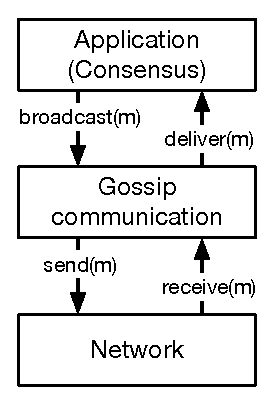
\includegraphics[width=0.3\columnwidth]{figures/modular.eps}
%\caption{Modular gossip design.}
%\label{fig:modular}
%\end{figure}

An algorithm interacts with the gossip communication layer using a {\em
broadcast} primitive that addresses a message to all \nodes. It is a
non-blocking primitive, as the dissemination is asynchronous and may take
several rounds.
The {\em deliver} primitive returns messages broadcast by \nodes. It is a
blocking primitive returning messages locally broadcast and messages received
from other \nodes.
%
There are no guarantees that a message broadcast by a non-faulty \node is
delivered by all non-faulty \nodes; due to \node  or link failures, a
message may never reach some destinations.
In addition, the random choice of peers to which messages are sent may not
provide full connectivity.
However, a proper choice of parameters provides very high reliability,
specially when the {\em push} dissemination strategy is adopted \cite{Birman99}.



\subsection{Tendermint}
\label{sec:Tendermint}

Tendermint \cite{buchman2019latestgossipbftconsensus} powers Cosmos, a network of proof-of-stake blockchains.
Both Tendermint and Cosmos are mature technologies, used by over a hundred businesses and running  on hundreds of computing nodes.
Tendermint builds an overlay network: a \node communicates directly with a restricted subset of \nodes, the node's neighbors or peers. 
To send a message to \nodes that are not its peers, a \node relies on gossip communication.

A \node is expected to maintain a long-term persistent identity in the form of a public key, from which the node's unique ID is derived. 
When attempting to connect to a peer \node, the first verifies whether the peer \node is in possession of the private key corresponding to its ID, thus preventing man-in-the-middle attacks. 
%To ensure liveness, 
We assume that each \node  is connected to at least $f+1$ peer \nodes, ensuring that at least one of the connected \nodes is honest. 

%\nm{This does not guarantee liveness; to guarantee liveness, you need to have the f+1-connected network, meaning that even if $f$ Byzantine replicas stop participating,
%the network will remain connected, and honest replicas will be able to communicate. To ensure a $f+1$ connected graph, each node having at least $f+1$ peers is necessary but insufficient.}   %\fd{Indeed, we are not checking this. I just omitted liveness from this discussion above.  Any idea how to proceed?.}

Tendermint runs a sequence of consensus instances.
An instance is also called a height and decides one block of transactions.
To decide a height, one to multiple attempts, called rounds, can be needed.

Nodes play the role of \textit{proposers} in the first round of successive heights of consensus
according to a function \textit{proposer(height, round)} known by all nodes.
To handle asynchrony and failures, a new round in the same height can be initiated and led by a different node.
%
Nodes also have voting power to accept (or not) blocks being proposed, acting as \textit{validators}.

%Each round has a validator leader, the round's proposer, and coordinator.  
Similar to PBFT's execution \cite{CL99:osdi}, composed of three steps, 
a failure-free round in Tendermint has the steps \textit{propose, prevote} and \textit{precommit}, briefly explained below for node \textit{n}.

\fp{The following fragment needs editing, as it doesn't naturally follow the text before. It'd be good if Daniel could double check this.}  \fd{reviewed this.}


\begin{description}[align=left]
\item[init] \textit{height=1, round=1};
\item[upon] \textit{n == proposer(height,round)}: broadcast \textsc{proposal} 
with a signed block of transactions and identification $id$;
\item[upon] receiving \textsc{proposal} from the current height and round's proposer: if the block can be accepted, sign and broadcast \textsc{prevote}.  Acceptance depends on further consensus rules and validation by the application;
\item[upon] receiving \textsc{proposal} and matching \textsc{prevote} messages from a quorum for the block $id$: broadcast a signed \textsc{precommit} message for the block $id$;
\item[upon] receiving \textsc{precommit} for the same block $id$ from a quorum: commit the block and append to the blockchain.   Deliver block's transactions to application and proceed to the next height, 1st round.  
\end{description}

Coherent with the proof-of-stake approach \cite{Poelstra2015DistributedCF}, nodes may have distinct voting power, that is, the vote of one node may have more weight than another.
A quorum is built by a subset of nodes aggregating more than $2/3$ of the total voting power.  

The straightforward description above is then enriched with additional rules to define whether a proposer must re-propose a block accepted in a previous round, and whether a node should accept the block proposed in a round.  The full algorithm can be found in \cite{buchman2019latestgossipbftconsensus}. 

%With equally distributed voting powers, this is the same as BFT quorums.   
%Validators with more voting power also become proportionally more frequent proposers.
% in the first round of new heights. 
%\nm{Do they become 
%proportionally more frequent proposers only in the first round of new heights or in general? I am not sure about this, but I think this is even true at the moment in Tendermint. } \fd{Not sure about this detail...  As we are not using this feature in the experiments, i just let the text generic in this regard.} 

The set of nodes is defined per consensus height.  The initial set is defined at the genesis state.  Then, modifications can be carried out with application commands.  The new set of nodes is proposed as an instance and is adopted if accepted.



